\documentclass[11pt,a4paper]{article}
\usepackage[utf8]{inputenc}
\usepackage[italian]{babel}
\usepackage{amsmath}
\usepackage{amsfonts}
\usepackage{amssymb}
\usepackage{array}
\usepackage{graphicx}
\usepackage{multirow}
\usepackage{color,colortbl}
\usepackage[hidelinks]{hyperref}
\usepackage{fancyhdr}
\usepackage{tabularx}
\usepackage[left=2cm,right=2cm,top=2cm,bottom=3cm]{geometry}
\usepackage{enumerate}
\usepackage{lastpage}
\usepackage{hyperref}
\usepackage{titlesec}
\usepackage{ltablex}
\hypersetup{colorlinks,urlcolor=blue,linkcolor=black}
\usepackage{listings}
\usepackage{multicol}
\setlength{\columnsep}{1cm}


\definecolor{lightgray}{rgb}{.9,.9,.9}
\definecolor{darkgray}{rgb}{.4,.4,.4}
\definecolor{purple}{rgb}{0.65, 0.12, 0.82}

\lstdefinelanguage{JavaScript}{
	keywords={typeof, new, true, false, catch, function, return, null, catch, switch, var, if, in, while, do, else, case, break},
	keywordstyle=\color{blue}\bfseries,
	ndkeywords={class, export, boolean, throw, implements, import, this},
	ndkeywordstyle=\color{darkgray}\bfseries,
	identifierstyle=\color{black},
	sensitive=false,
	comment=[l]{//},
	morecomment=[s]{/*}{*/},
	commentstyle=\color{purple}\ttfamily,
	stringstyle=\color{red}\ttfamily,
	morestring=[b]',
	morestring=[b]"
}

\lstset{
	language=JavaScript,
	backgroundcolor=\color{lightgray},
	extendedchars=true,
	basicstyle=\footnotesize\ttfamily,
	showstringspaces=false,
	showspaces=false,
	numbers=left,
	numberstyle=\footnotesize,
	numbersep=9pt,
	tabsize=2,
	breaklines=true,
	showtabs=false,
	captionpos=b
}

\renewcommand{\lstlistingname}{Esempio}% Listing -> Algorithm
\renewcommand{\lstlistlistingname}{Elenco degli Esempi}% List of Listings -> List of Algorithms

\pagestyle{fancy}
\fancyhf{}
\lhead{
\includegraphics[scale=0.07]{images/logo.png}}

\renewcommand {\footrulewidth}{0.2mm}
\lfoot {Manuale Utente}
\rfoot{Pagina \thepage\ di \pageref{LastPage}}

\definecolor{LightBlue}{rgb}{0,0,0.5}
\definecolor{Gray}{gray}{0.8}
\definecolor{LightGray}{gray}{0.9}

\usepackage{lipsum}
\usepackage{verbatim}


\setcounter{tocdepth}{4}
\setcounter{secnumdepth}{4}

\titlespacing*{\subsection}{0pt}{8ex plus 1ex minus .2ex}{2.3ex plus .2ex}
\titlespacing*{\subsubsection}{0pt}{8ex plus 1ex minus .2ex}{2.3ex plus .2ex}

\begin{document}
	\begin{titlepage}
  \centering
	\scshape
	
	\vspace*{2cm}
	
\includegraphics[scale=0.7]{images/logo.png}
	\rule{\linewidth}{0.2mm}\\[0.37cm]
	{\Huge Piano di progetto}\\
	\rule{\linewidth}{0.2mm}\\[1cm]
	{\LARGE\bfseries Progetto Colletta - Gruppo OttoBit}\\[1cm]
	
	
	
	\begin{tabular}{>{\columncolor{Gray}}r | >{\normalfont}l}
		\rowcolor{LightBlue}		
		\multicolumn{2}{c}{\color{white}{Informazioni sul documento}}\\
		Versione & 1.0.0 \\
		Redazione & Benedetto Cosentino\\
							& Enrico Marcato\\
 		Verifica & Giovanni Peron\\
 		Responsabile & Benedetto Cosentino\\
 		Uso & Esterno\\
 																 		& Prof. Tullio Vardanega\\
 																		& Prof. Riccardo Cardin\\
 		\multirow[t]{-3}{*}{Destinatari}	& MIVOQ s.r.l\\
 		\hline
	\end{tabular}
\end{titlepage}
	
	{\def\arraystretch{2}\tabcolsep=10pt
	\newpage
	\section*{\centering Registro delle modifiche}
	\begin{tabularx}{\textwidth}{ c | c | p{3.80cm} | c | X }
		\rowcolor{LightBlue}
		\color{white}\bfseries Versione & \color{white}\bfseries Data & \multicolumn{1}{c}{\color{white}\bfseries Autore}
		& \color{white}\bfseries Ruolo & \multicolumn{1}{c}{\color{white}\bfseries Descrizione}\\[0.25cm]
		1.0.0 & 2019-04-11 & Eleonora Peagno & Responsabile & Approvazione per il \newline rilascio \\ \hline
		0.2.0 & 2019-04-11 & Giovanni Peron & Verificatore & Verifica documento \\ \hline
		0.1.2 & 2019-04-11 & Enrico Marcato & Progettista & Sistemazione requisiti e immagini \S3 \\ \hline
		0.1.1 & 2019-04-11 & Enrico Marcato & Progettista & Aggiunte funzionalità \S3  \\ \hline
		0.1.0 & 2019-04-11 & Giovanni Bergo & Verificatore & Verifica documento \\ \hline
		0.0.2 & 2019-04-07 & Enrico Marcato & Progettista & Redatto \S2 e \S3 \\ \hline
		0.0.1 & 2019-04-05 & Enrico Marcato & Progettista & Creazione documento e stesura \S1 \\ 
	 \hline		
	\end{tabularx}
	
	\newpage	
	
	\renewcommand  \contentsname {\Large Indice} 
	
	\tableofcontents
	\newpage
	\listoffigures

	\newpage
	
	\section{Introduzione}
	\subsection{Scopo del documento}
	Lo scopo di questo documento è quello di illustrare le funzionalità che l'applicazione possiede e spiegarne l'utilizzo. Esso rappresenta una guida per l'utilizzo del prodotto.
	\subsection{Scopo del prodotto}
	Lo scopo del prodotto è creare una piattaforma collaborativa di raccolta dati su cui sia possibile predisporre e/o svolgere esercizi di analisi grammaticale. La raccolta vorrebbe avere il fine di fornire a sviluppatori e ricercatori dati sufficienti per applicare metodi di apprendimento automatico$^*$. Nello specifico si vorrebbe poter insegnare ad un elaboratore a svolgere gli stessi esercizi proposti agli utenti, divenendo una sorta di correttore automatico.
	
	\subsection{Note esplicative}
	Tutti i termini marcati con un * ad apice presenti nel seguente documento trovano una definizione
	nell'appendice in fondo al documento.
	I nomi dei documenti interni/esterni prodotti dal gruppo OttoBit saranno scritti in corsivo.
	\newpage
	\section{Download e installazione}
	\subsection{Requisiti}
	L'applicazione è supportata solo ed esclusivamente da dispositivi desktop. In seguito illustriamo i requisiti richiesti per il funzionamento di Colletta.
	\subsubsection{Sistemi operativi:} 
	\paragraph{Windows}
	\begin{itemize}
		\item Sistema: Windows 7, 8 or 10, 32-bit or 64-bit
		\item RAM: 1GB
		\item Hard-drive: 1GB di spazio
		\item Connessione ad Internet: obbligatoria
	\end{itemize}
	\paragraph{Linux}
	\begin{itemize}
		\item Sistema: Ubuntu 17.10
		\item RAM: 512MB
		\item Hard-drive: 1GB di spazio
		\item Connessione ad Internet: obbligatoria
	\end{itemize}
	\paragraph{Mac}
	\begin{itemize}
		\item Sistema: MacOS Mojave 10.14.4
		\item RAM: 512MB
		\item Hard-drive: 1GB di spazio
		\item Connessione ad Internet: obbligatoria
	\end{itemize}
	\subsubsection{Browser:}
		\begin{itemize}
		\item Mozilla Firefox 66.0;
		\item Google Chrome 67.0;
		\item Safari 12.1 (solo per MacOS).		
	\end{itemize}
	\subsubsection{Framework:}
		\begin{itemize}
		\item NodeJS*.
		\end{itemize}
	

	\subsection{Download}
	\subsubsection{NodeJS}
	Scaricare NodeJS per il sistema operativo desiderato da \url{https://nodejs.org/en/download}.
	\subsubsection{Colletta}		
	L'applicazione è disponibile alla seguente repository Github:
	\url{https://github.com/ottoBitPd/colletta-poc}.
	
	\subsection{Installazione}
	La piattaforma è provvisoriamente raggiungibile solo tramite server locale.
	Per creare un server locale, eseguire i seguenti passaggi:
	 \begin{enumerate}
	 	\item \textbf{Installare le librerie necessarie:}\\ Posizionarsi nella cartella principale, aprire la shell e utilizzare il seguente comando:\begin{lstlisting}[numbers=none]
	 	npm install
	 	\end{lstlisting}
	 	\item \textbf{Eseguire il server:}\\ Sempre da terminale e nella cartella principale, utilizzare il seguente comando:\begin{lstlisting}[numbers=none]
	 	node public/index.js
	 	\end{lstlisting}
	 	\item \textbf{Accedere all'applicazione:}\\ Apri il tuo browser e vai all'indirizzo: \url{http://localhost:8080}
	 \end{enumerate}
 
 \newpage
	\section{Utilizzo}	
	
	\subsection{Primo accesso alla piattaforma}
	La prima schermata che appare una volta entrati nella piattaforma è considerata l'homepage (vedi Figura 1). Nella quale è possibile accedere alle funzionalità di registrazione, autenticazione e di ricerca o aggiunta di un esercizio.
	
	\begin{figure}[h]
		\centering
		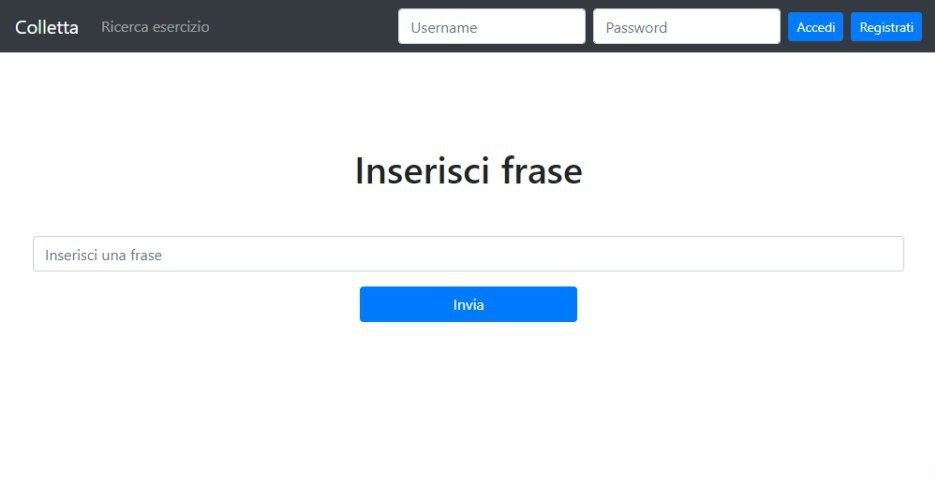
\includegraphics[scale=0.65]{images/home.jpg}
		\caption{Homepage}
	\end{figure}
	
	\subsection{Registrazione}
	Per registrarsi a Colletta seguire i seguenti passi:
	\begin{enumerate}
	\item Accedere all'homepage e cliccare su "Registrati";
	\item Scegliere se registrarsi come allievo oppure come insegnante;
	\item Compilare i campi richiesti;
	\item Se è stata scelta l'opzione allievo cliccare su "Registrati" e la registrazione è conclusa.
	\item Se è stata scelta la registrazione come insegnante cliccare su "Registrati" e attendere che un moderatore accetti la richiesta.
	\end{enumerate}

	\begin{figure}[h]
		\centering
		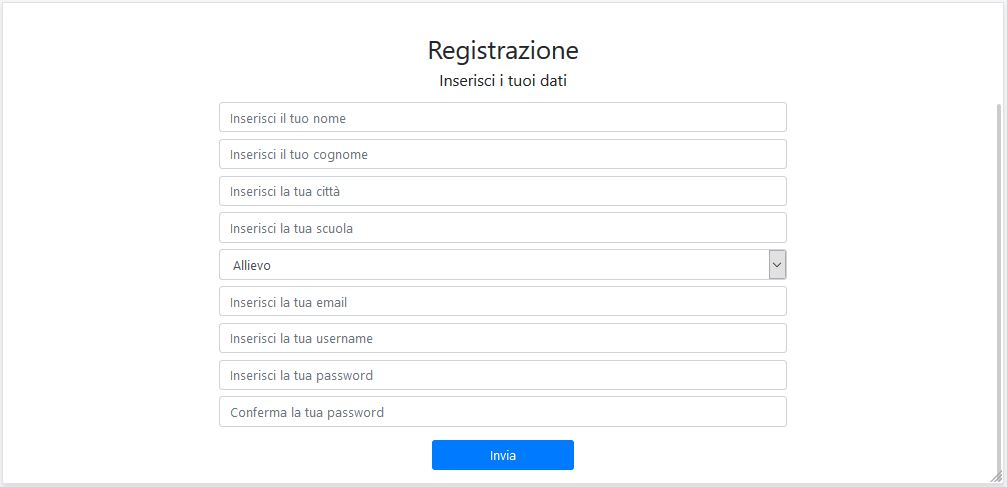
\includegraphics[scale=0.65]{images/registrazione.jpg}
		\caption{Registrazione}
	\end{figure}
	\newpage

	\subsection{Autenticazione}
	Per accedere a Colletta come allievo o insegnante seguire i seguenti passi:
	\begin{enumerate}
		\item Accedere all'homepage (vedi Figura 1);
		\item Compilare con le credenziali username e password i campi nella navbar;
		\item Cliccare su "Accedi".
	\end{enumerate}

	\subsection{Inserimento frase}
	Inserire una frase permette di eseguire un esercizio non presente nella piattaforma e ricevere la valutazione automatica quindi non inserita da un insegnante.	
	\begin{enumerate}
		\item Accedere all'homepage (vedi Figura 1);
		\item Inserire la frase desiderata nella barra;
		\item Cliccare su "Invia";
	\end{enumerate}

	\newpage
	\subsection{Ricerca esercizio}
	La ricerca avviene tra esercizi aggiunti precedentemente da insegnanti. 
	
	\begin{enumerate}
		\item Accedere all'homepage e cliccare su "Ricerca esercizio" nella navbar;
		\item Nell'elenco di tutti gli esercizi è possibile selezionare quale svolgere cliccando su "Esegui esercizio";
		\item Per filtrare gli esercizi, inserire la frase desiderata nella barra;
		\item Cliccare su "Cerca";
	\end{enumerate}
	
	\begin{figure}[h]
		\centering
		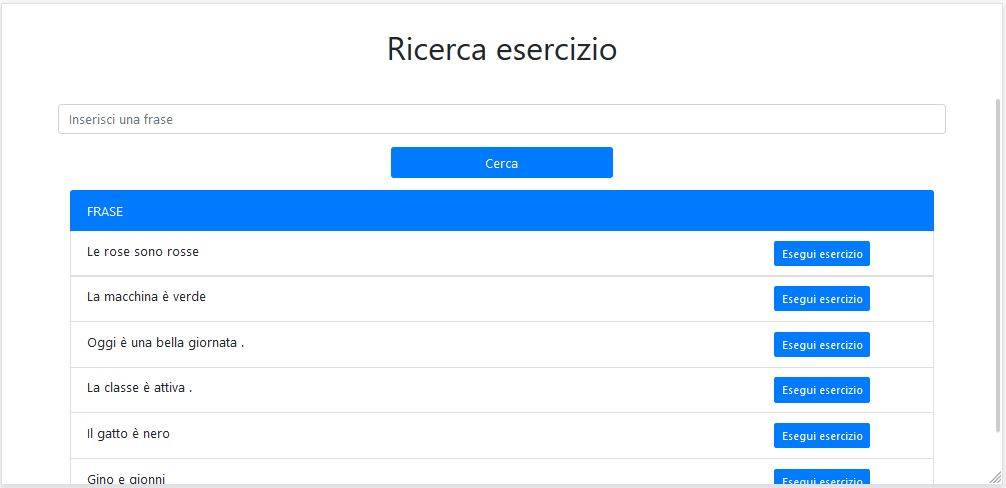
\includegraphics[scale=0.65]{images/ricerca.jpg}
		\caption{Ricerca esercizio}
	\end{figure}
	
	\subsection{Svolgimento esercizio}
	\begin{enumerate}
		\item Accedere all'homepage e svolgere Inserimento frase(\S3.4) oppure Ricerca esercizio(\S3.5);
		\item Compilare i campi opportunamente;
		\item Scegliere l'autore della correzione;
		\item Cliccare su "Invia".
	\end{enumerate}

	\begin{figure}[h!]
		\centering
		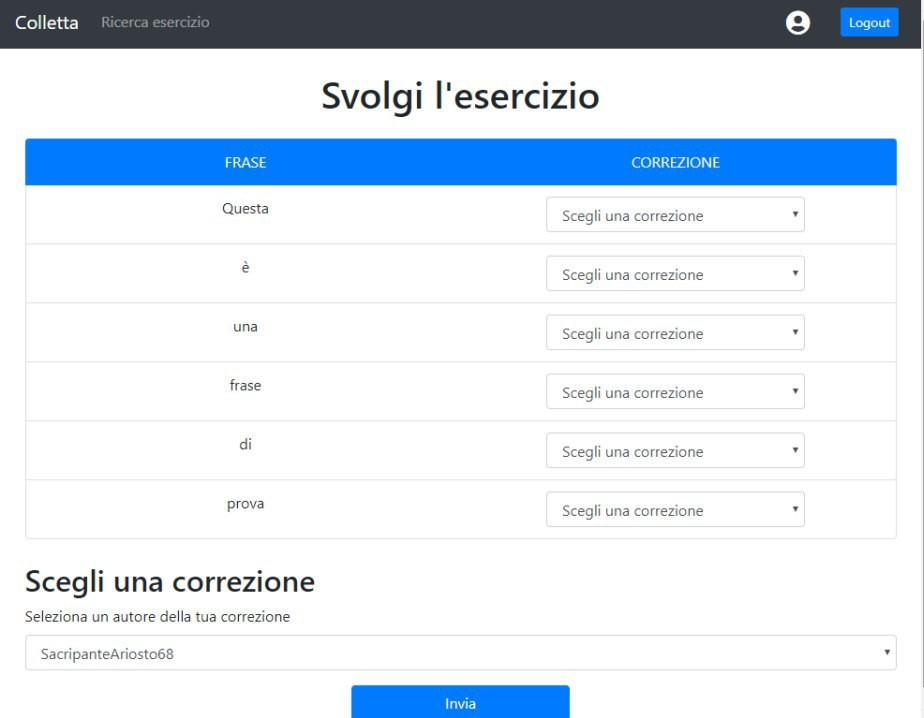
\includegraphics[scale=0.65]{images/svolgimento.jpg}
		\caption{Svolgimento esercizio}
	\end{figure}
	
	\newpage
	
	\subsection{Valutazione esercizio}
	Al termine dell'esercizio vengono evidenziati eventuali errori in rosso e in verde le soluzioni esatte.
		\begin{figure}[h!]
		\centering
		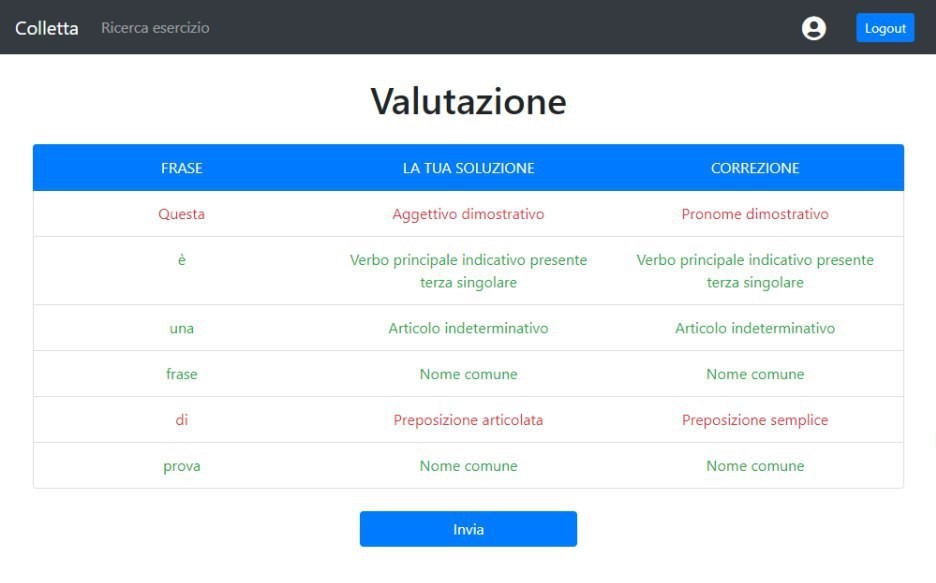
\includegraphics[scale=0.65]{images/valutazione.jpg}
		\caption{Valutazione}
	\end{figure}
	
	\subsection{Visualizzare e modificare la informazioni del profilo}
	Sia gli allievi che gli insegnanti hanno la possibilità di visualizzare e modificare le proprie informazioni personali:
	\begin{enumerate}
		\item Autenticarsi e cliccare sull'icona del profilo nella navbar;
		\item Modificare se necessario compilando i campi;
		\item Clicca su "Modifica".
	\end{enumerate}

	\begin{figure}[h]
		\centering
		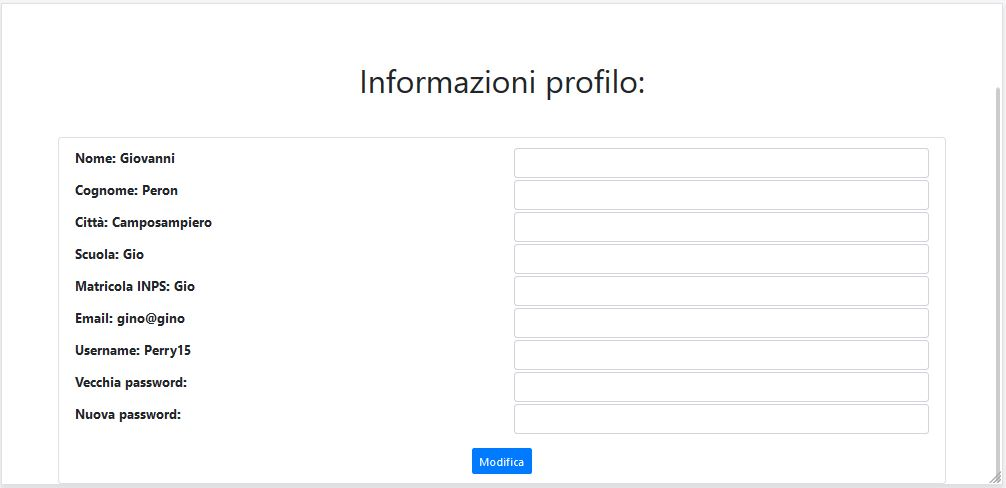
\includegraphics[scale=0.65]{images/profiloinsegnante.jpg}
		\caption{Profilo insegnante}
	\end{figure}
	
	\newpage
	\subsection{Visualizzare i progressi}
	Questa funzionalità è riservata all'utente di tipo \textbf{Allievo}.\\
	In questa pagina sono rappresentati i progressi dell'alunno ricavati dagli esercizi svolti suddivisi per settimana.
	
	\begin{enumerate}
		\item Autenticarsi e cliccare sull'icona del profilo nella navbar;
		\item Cliccare su "I tuoi progressi" nella navbar;
	\end{enumerate}

	\begin{figure}[h]
		\centering
		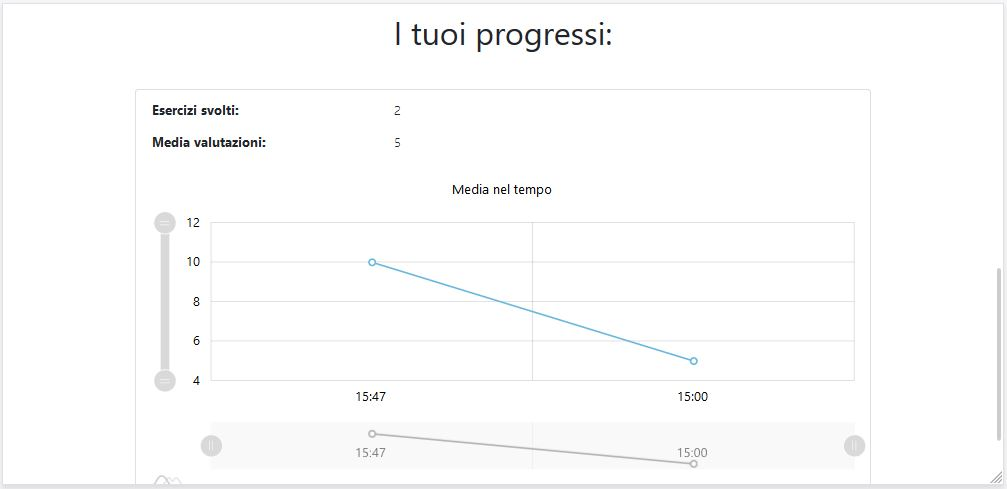
\includegraphics[scale=0.65]{images/progressi.jpg}
		\caption{Progressi alunno}
	\end{figure}	
	
	\newpage
	\subsection{Svolgere esercizi assegnati}
	Questa funzionalità è riservata all'utente di tipo \textbf{Allievo}.
	
	\noindent Un insegnante assegna esercizi ad una classe, gli alunni appartenenti ad essa possono svolgerli seguendo i seguenti passi:
	
	\begin{enumerate}
		\item Autenticarsi e cliccare su "Le tue classi" nella navbar;
		\item Cliccare sulla classe desiderata;
		\item Nell'elenco degli esercizi assegnati alla classe cliccare su "Esegui esercizio" per selezionare l'esercizio da svolgere.
	\end{enumerate}

	\begin{figure}[h]
		\centering
		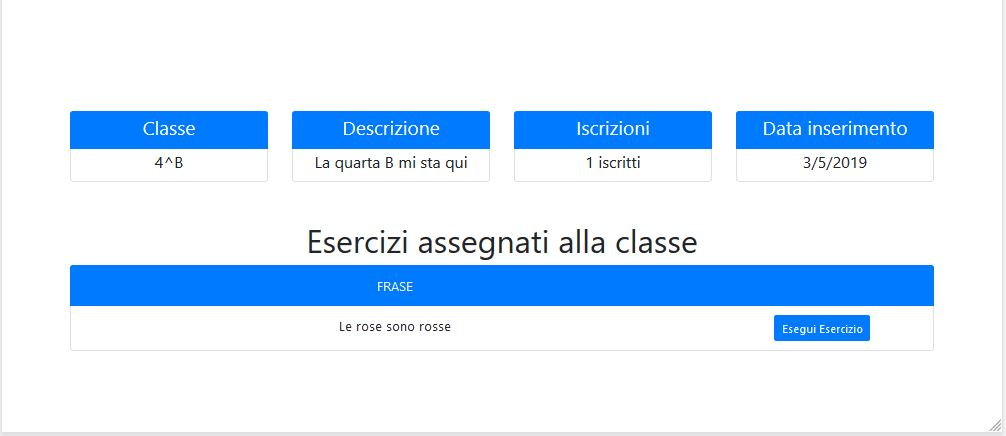
\includegraphics[scale=0.65]{images/esassegnato.jpg}
		\caption{Svolgimento esercizio assegnato}
	\end{figure}
		
	\newpage
	\subsection{Inserire una frase e fornire una soluzione}
		Questa funzionalità è riservata all'utente di tipo \textbf{Insegnante}.
		
		\noindent Un insegnante per inserire un esercizio nella piattaforma deve inserire una frase e la corrispondente soluzione.
		
		\begin{enumerate}
			\item Autenticarsi e cliccare su "Crea esercizio" nella navbar;
			\item Completa la barra con la frase da inserire, poi clicca su "Invia";
			\item Nella soluzione proposta dall'apprendimento automatico, modifica i campi che non ritieni giusti corretti
			\item Cliccare su "Invia". 
		\end{enumerate}
	
		\begin{figure}[h]
			\centering
			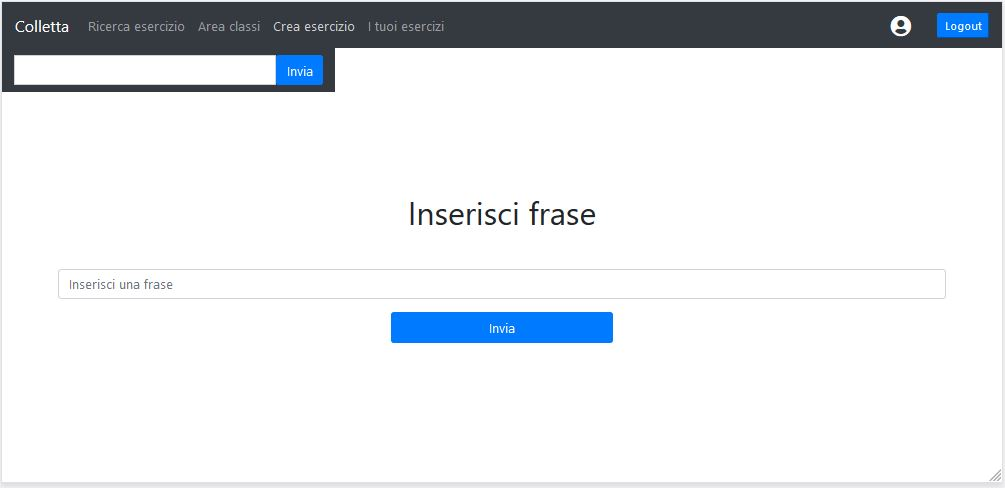
\includegraphics[scale=0.65]{images/creaes.jpg}
			\caption{Creazione nuovo esercizio}
		\end{figure}

	\subsection{Creare una classe}
		Questa funzionalità è riservata all'utente di tipo \textbf{Insegnante}.\\
		Una classe permette ad un insegnante di interagire direttamente con i propri allievi.
		
			\begin{figure}[h!]
				\centering
				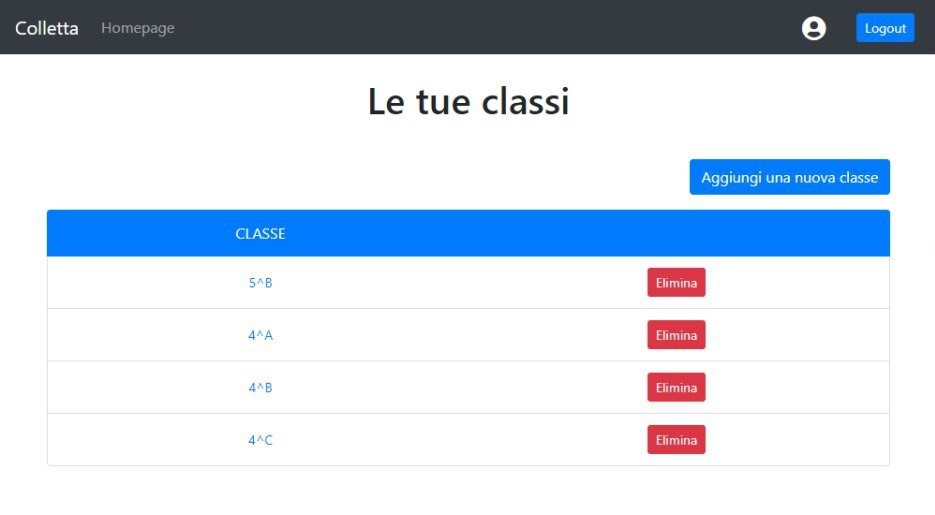
\includegraphics[scale=0.65]{images/classi.jpg}
				\caption{Gestione delle classi}
			\end{figure}
	
		\begin{enumerate}
			\item Autenticarsi e cliccare su "Area classi" nella navbar;
			\item Cliccare su "Aggiungi una nuova classe";
			\item Compilare i campi dati richiesti;
			\item Clicca su "Crea classe";
		\end{enumerate}
	
	\subsection{Assegnare esercizio ad una classe}
		Questa funzionalità è riservata all'utente di tipo \textbf{Insegnante}.\\
		Assegnando esercizi ad una classe si permette agli allievi appartenti alla stessa di svolgere tali esercizi.
		
		\noindent \textbf{Attenzione:} l'esercizio che verrà assegnato deve essere già esistente.
		
		\begin{enumerate}
			\item Autenticarsi e cliccare su "Area classi" nella navbar;
			\item Cliccare sulla classe desiderata;
			\item Cliccare su "Assegna un nuovo esercizio".
			\item Ricercare un esercizio già esistente;
			\item Cliccare su "Aggiungi esercizio alla classe";
		\end{enumerate}
		
		\subsection{Assegnare allievo ad una classe}
		Questa funzionalità è riservata all'utente di tipo \textbf{Insegnante}.\\
		Assegnando un allievo ad una classe si permette all'allievo di essere valutato negli esercizi assegnati alla stessa classe.
		
		\begin{enumerate}
			\item Autenticarsi e cliccare su "Area classi" nella navbar;
			\item Cliccare sulla classe desiderata;
			\item Cliccare su "Aggiungi uno studente".
			\item Ricercare lo studente desiderato;
			\item Cliccare su "Aggiungi alla classe".
		\end{enumerate}
	
		\begin{figure}[h!]
		\centering
		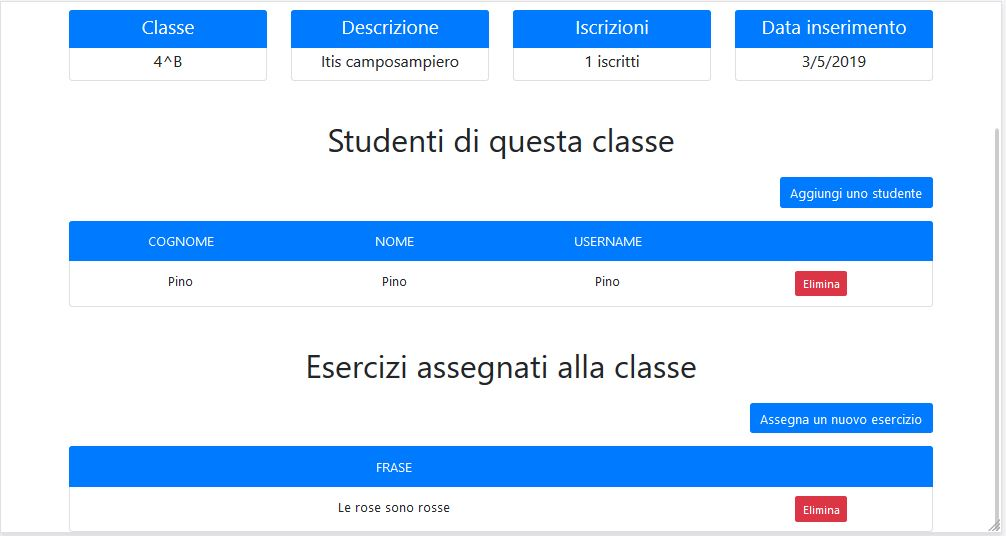
\includegraphics[scale=0.65]{images/gestioneclasse.jpg}
		\caption{Gestione della singola classe}
	\end{figure}
			
	\newpage

	\subsection{Autenticazione riservata allo sviluppatore}
		Questa funzionalità è riservata all'utente di tipo \textbf{Sviluppatore}.\\
		
	\noindent	Lo sviluppatore ha accesso alla visione dei dati presenti nella piattaforma con inoltre la possibilità di filtrarli e scaricarli in diversi formati.\\ Per accedere a questa area seguire i seguenti passi:\\
		
	\noindent	\textbf{Attenzione:} Lo sviluppatore deve essere in possesso della password consegnata dai possessori della piattaforma.
		
		\begin{enumerate}
			\item Accedere alla homepage della piattaforma;
			\item Aggiungere "/developer" all'url e premere invio;
			\item Inserire la password;
			\item Premere "Invia".
		\end{enumerate}
	
	\begin{figure}[h]
		\centering
		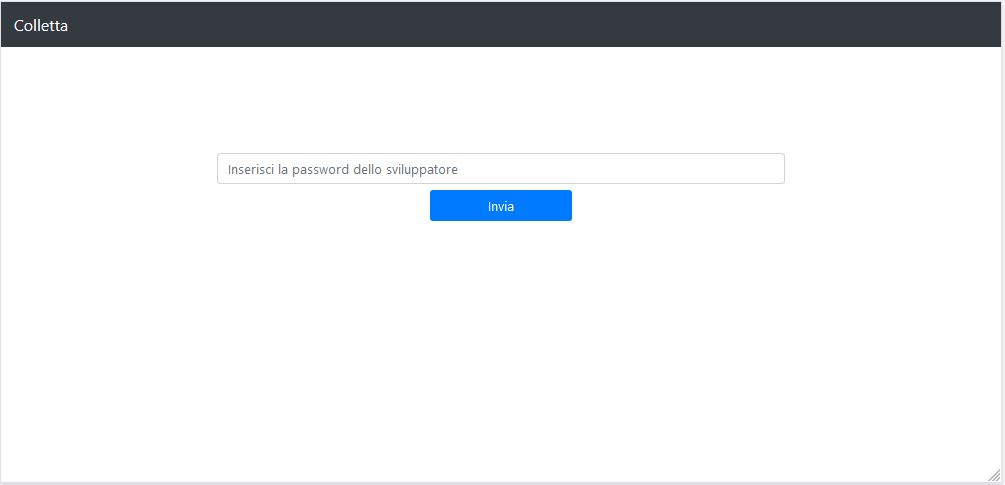
\includegraphics[scale=0.65]{images/homesviluppatore.jpg}
		\caption{Autenticazione sviluppatore}
	\end{figure}

	\newpage
	\subsection{Filtraggio dati}
		Questa funzionalità è riservata all'utente di tipo \textbf{Sviluppatore}.
		\\ \\
		Lo sviluppatore può filtrare i dati riguardanti un esercizio inserendo una valutazione minima e/o massima con le date riguardanti un ristretto periodo di tempo . Ogni utente registrato per questioni relative alla privacy è riconoscibile dallo sviluppatore solamente tramite un hash. Se lo sviluppatore individua personalmente un utente che ritiene affidabile, inserendo il suo codice hash può filtrare gli esercizi da lui eseguiti.
		
		\begin{enumerate}
			\item Accedere alla piattaforma e autenticarsi;
			\item Compilare i campi necessari per la ricerca dei dati;
			\item Cliccare su "Filtra".
		\end{enumerate}
	

		\begin{figure}[h]
		\centering
		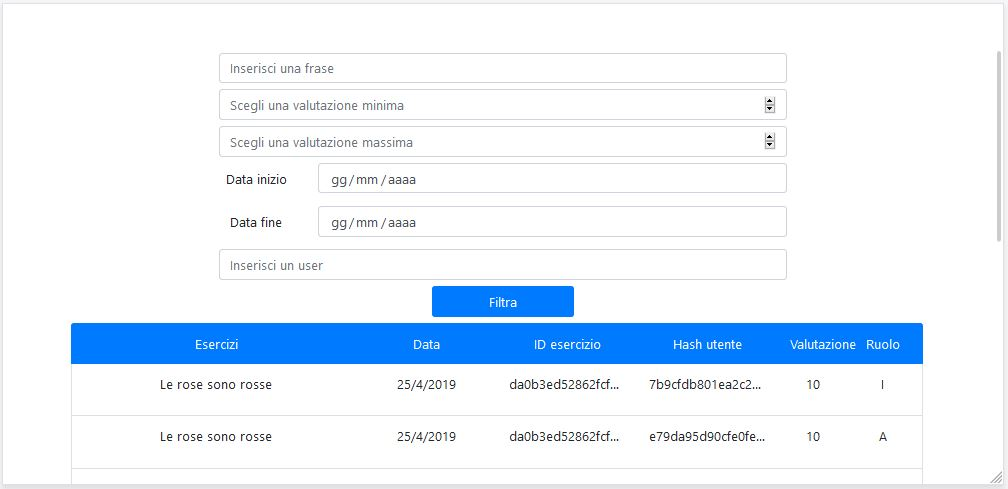
\includegraphics[scale=0.65]{images/filtrodati.jpg}
		\caption{Filtraggio dati}
		\end{figure}
		
	
	\newpage
	
	\subsection{Scaricare modello}
		Questa funzionalità è riservata all'utente di tipo \textbf{Sviluppatore}.\\
		
		\begin{enumerate}
			\item Accedere alla piattaforma e autenticarsi;
			\item Cliccare su "Scarica modello".
		\end{enumerate}
	
	\begin{center}
	\begin{figure}[h]
		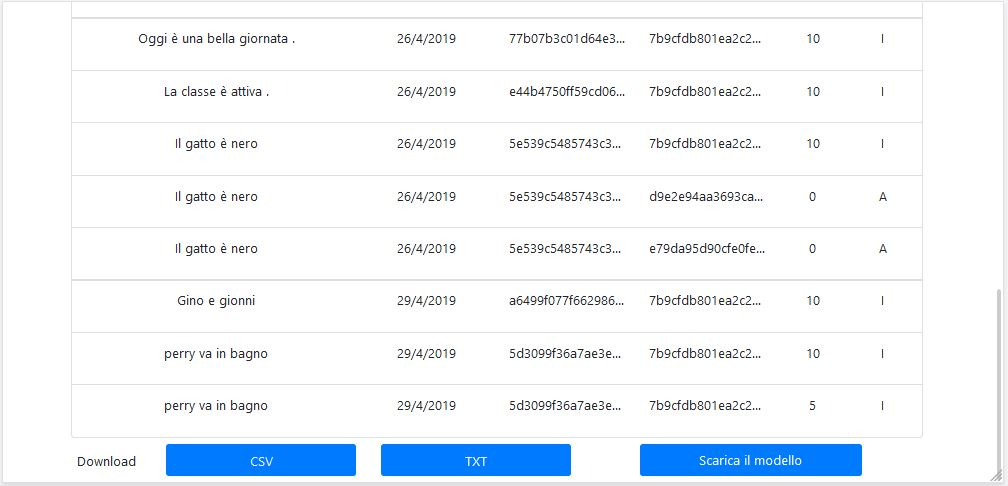
\includegraphics[scale=0.65]{images/scaricamodello.jpg}
		\caption{Download modello}
	\end{figure}
\end{center}
				
	\subsection{Scaricare dati}
		Questa funzionalità è riservata all'utente di tipo \textbf{Sviluppatore}.\\
	
		I dati sono disponibili al download in formato csv e txt.
		\begin{enumerate}
			\item Accedere alla piattaforma e autenticarsi;
			\item Se necessario filtrare i dati di interesse (\S3.17);
			\item Cliccare su "CSV" o "TXT".
		\end{enumerate}

\newpage

\appendix
\setcounter{secnumdepth}{0}
\section{Glossario}
	\subsection*{A}
		\subsubsection*{Apprendimento automatico}
	L'apprendimento automatico rappresenta un insieme di meccanismi che permettono ad un calcolatore
	di migliorare nel tempo l'esecuzione di un esercizio.
	
	\subsection*{N}
		\subsubsection*{NodeJS}
	Node.js è una runtime di JavaScript Open source multipiattaforma orientato agli eventi per l'esecuzione di codice JavaScript Server-side.
	


\end{document}

